\documentclass[tikz,border=2pt]{standalone}
\usepackage{amsmath,amssymb}
\usepackage{tikz}
\usetikzlibrary{arrows.meta}

\begin{document}
% z - w is the arrow from w to z; translated to start at the origin it is (a-c) + (b-d)i.
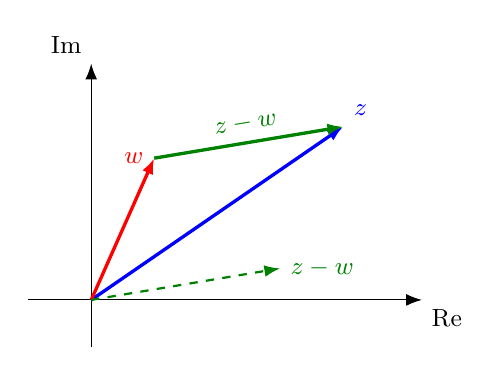
\begin{tikzpicture}[every node/.style={font=\small}, >={Latex[length=2mm]}]
	\draw[->] (-0.8,0) -- (4.2,0) node[below right] {$\mathrm{Re}$};
	\draw[->] (0,-0.6) -- (0,3.0) node[above left] {$\mathrm{Im}$};
	\draw[->, blue, very thick] (0,0) -- (3.2,2.2) node[above right] {$z$};
	\draw[->, red, very thick] (0,0) -- (0.8,1.8) node[left] {$w$};
	\draw[->, green!50!black, very thick] (0.8,1.8) -- (3.2,2.2) node[midway, above, sloped] {$z-w$};
	\draw[->, green!50!black, thick, dashed] (0,0) -- (2.4,0.4) node[right] {$z-w$};
\end{tikzpicture}
\end{document}
